\documentclass[conference]{IEEEtran}
\IEEEoverridecommandlockouts
% The preceding line is only needed to identify funding in the first footnote. If that is unneeded, please comment it out.
\usepackage{cite}
\usepackage{amsmath,amssymb,amsfonts}
\usepackage{algorithmic}
\usepackage{graphicx}
\usepackage{textcomp}
\usepackage{xcolor}
\usepackage[nolist]{acronym}
\usepackage{subcaption}
\usepackage{tikz}
\usepackage{pgfplots}
\usepackage[font=footnotesize]{caption}        % small, footnotesize, scriptsize, or large
\captionsetup[figure]{labelfont={bf}}
\pgfplotsset{compat=1.18}
\acresetall
\def\BibTeX{{\rm B\kern-.05em{\sc i\kern-.025em b}\kern-.08em
    T\kern-.1667em\lower.7ex\hbox{E}\kern-.125emX}}

\begin{acronym}[SPS] % longest acronym in [...] for spacing
    \acro{AVX}{advanced vector extensions}
    \acro{CPU}{central processing unit}
    \acro{DAG}{directed acyclic graph}
    \acro{GPU}{graphics processing unit}
    \acro{HZB}{hierarchical z-buffering}
    \acro{PM}{per-meshlet}
    \acro{SIMD}{single instruction multiple data}
    \acro{SVO}{sparse voxel octree}
    \acro{TPOC}{two-pass occlusion culling}
    \acro{TPOC-PM}{two-pass occlusion culling - per-meshlet}
    \acro{TPOC-PON}{two-pass occlusion culling - per-octree-node}

    % acrodefplural, wenn eine Pluralform benötigt wird (Standard: angehängtes "s" aus dem Englischen)
    % \acrodefplural{acroKey}[plural short]{plural long}
\end{acronym}

\begin{document}

\title{Two-Pass Occlusion Culling for Dynamic Voxel Scenes based on Hierarchical Z-Buffering\\}

\author{
    
    \IEEEauthorblockN{1\textsuperscript{st} Frederik Omlor}
    \IEEEauthorblockA{\textit{Department of Computer Science} \\
    \textit{Media University Stuttgart}\\
    Stuttgart, Germany \\
    fo025@hdm-stuttgart.de}
    *Corresponding author
    ~\\
    \and
    \IEEEauthorblockN{2\textsuperscript{nd} Stefan Radicke}
    \IEEEauthorblockA{\textit{Department of Computer Science} \\
    \textit{Media University Stuttgart}\\
    Stuttgart, Germany \\
    radicke@hdm-stuttgart.de}
    ~\\
    \and
    \IEEEauthorblockN{3\textsuperscript{rd} Andreas Stiegler}
    \IEEEauthorblockA{\textit{Research and Development} \\
    \textit{Strichpunkt Design}\\
    Stuttgart, Germany \\
    a.stiegler@sp.design}
    ~\\
    \and[\hfill\mbox{}\par\mbox{}\hfill]
    \IEEEauthorblockN{4\textsuperscript{th} Wilhelm Lorin Atzberger}
    \IEEEauthorblockA{\textit{Senior Graphics Engineer} \\
    \textit{Unity Technologies}\\
    Copenhagen, Denmark \\
    lorin.atzberger@gmail.com}
}

\maketitle

\begin{abstract}
    We present two-pass occlusion culling (TPOC) for dynamic voxel scenes based on hierarchical 
    z-buffering (HZB). Our approach to TPOC uses larger geometry as an approximation of the scene's 
    volume and can be applied to a scene that not only approximates the surface by using voxels 
    but also includes a voxel-based volume that might be exposed or altered during runtime. A great 
    amount of the algorithm relies on GPU-driven computations, which allow for millions of voxels 
    to be drawn efficiently. The HZB algorithm has recently gained popularity due to its ability 
    to efficiently cull occluded geometry using a GPU-driven approach. This algorithm has not been 
    available in its original form for dynamic voxel-based scenes. Our TPOC implementation uses an 
    octree to efficiently schedule voxel data with respect to their spatial characteristics and 
    replaces full octree nodes with larger geometry for fast computation of the HZB. This not only 
    allows the application of HZB to a dynamic voxel scene, but also results in increased performance 
    up to 90\% compared to a rendering pipeline without occlusion culling. We show that the use of 
    the mesh shading pipeline in combination with a sparse voxel octree (SVO) can adapt the HZB to 
    efficiently occlude a significant number of voxels, resulting in an overall performance increase 
    of up to 42\% as compared to a per-octree-node culling approach.
\end{abstract}

\begin{IEEEkeywords}
occlusion culling, hierarchical z-buffering, voxel rendering, mesh shading
\end{IEEEkeywords}

\section{Introduction}

\noindent
Real-time voxel rendering usually has two distinct fields of application: real-time 
raytracing and the traditional rasterized rendering approach. While the former is 
popular due to the uniform nature of voxels and the ability to easily cast rays using 
a regular voxel grid, the latter has been used in real-time applications for volumetric 
representations of scenes and simple physics or similar dynamic interactions \cite{b9, b10}. \\

\noindent
Over the last decades, ray tracing has been subject to a lot of innovation, especially in  
real-time applications for entertainment purposes, i.e., games. Hardware manufacturers have 
been adding more support for specific raytracing compute units, and the software side of 
\ac{GPU}s has been upgraded to support features like ray-traced ambient occlusion, shadows, 
and global illumination. However, the rasterized approach to voxel rendering  has not been 
very present in the entertainment industry, although the rasterized rendering pipeline has 
been upgraded significantly over the last decade. A central overhaul is the mesh shading 
pipeline, which has been introduced to \ac{GPU}s in 2018. It features a new way of preprocessing 
vertices using a more general compute architecture that allows for more efficient \ac{GPU} 
computations \cite{b11}. \\

\noindent
Recent games made use of \ac{HZB} in combination with the mesh shading pipeline to efficiently 
cull mesh instances and even invisible parts of meshes. While the original algorithm by Greene 
et al. \cite{b1} was intended to be used on the \ac{CPU}, modern applications of \ac{HZB} are 
implemented as \ac{GPU}-driven occlusion culling techniques, which have been a driving factor 
for the recent increase in geometrical density \cite{b12, b13}. The approach is heavily reliant on the presence 
of large, static occluder geometry, which makes it inefficient to be used in voxelized scenes 
in the form it has been so far. \\

\noindent
In this paper, we present a technique to dynamically approximate volumetric voxel scenes, and 
show that the use of the mesh shading pipeline in combination with a \ac{SVO} can adapt the 
\ac{HZB} to efficiently occlude a significant number of voxels, which results in an overall 
performance increase. The term volumetric voxel scene refers to a scene that not only 
approximates the surface by using voxels but also includes a voxel-based volume that might be 
exposed or altered during runtime. A great amount of the algorithm relies on \ac{GPU}-driven 
computations, which allow for millions of voxels to be drawn efficiently. \\

\noindent
Our technique is based on the assumption that a vast amount of voxels within and behind a given 
part of the scene is occluded by some other voxels in the same scene. The technique approximates 
the non-visible volume within a voxel scene and uses it as an occluder for \ac{GPU}-based \ac{HZB}. 
We have implemented and tested the algorithm in two different configurations:

\begin{itemize}
    \item \ac{TPOC-PM} using a mesh shading pipeline; testing individual meshlets for occlusion 
    \item \ac{TPOC-PON} using a mesh shading pipeline; testing individual octree nodes for occlusion
\end{itemize}

\section{Related Work}

\subsection{Voxel Scene Representations} \label{subsec-voxel-scn-rep}

\noindent
Laine and Karras \cite{b6} present a variation of the base \ac{SVO} approach for efficiently 
ray tracing voxel models. In their work, contours are used to approximate octree nodes within 
a \ac{SVO}. If the octree node is found to be approximated good enough, the subdivision to 
deeper levels in the octree node is terminated. This way, \ac{SVO}s can be significantly 
reduced in size, which benefits the memory footprint of the application and aims to increase 
real-time raytracing performance. Laine and Karras show that the use of contours can increase 
the ray casting performance by approximately $77\%$. Using an additional optimization technique 
for approximating the ray casting starting porition, they were able to further increase casting 
performance by another $12\%$.  \\

\noindent
Kämpe et al. \cite{b2} propose the use of their high-resolution sparse voxel \ac{DAG}. 
This approach is tailored to high voxel resolutions and data that might not fit into 
memory all at once. Their data structure can be easily split up into several subtrees, 
which in turn can be loaded individually. This approach seems promising for large scenes 
and use cases, which require the streaming of data. They propose to structure the data in 
a way that enables equal nodes of an octree hierarchy to be reduced to only one instance, 
eliminating redundant parts of the hierarchy and reducing the amount of used memory by up 
to $38\times$ compared to similar voxel representations. \\

\noindent
Our approach makes use of an \ac{SVO} for storing the voxels in respect to their spatial 
characteristics. Although we implemented a custom \ac{SVO}, our approach to \ac{TPOC} for 
voxel scenes can benefit from using a high-resolution sparse voxel \ac{DAG} for even larger 
voxel counts.

\subsection{Occlusion Culling} \label{subsec-occlusion-culling}

\noindent
Greene et al. \cite{b1} proposed the first \ac{HZB} algorithm with the capability to use 
screen space data to cull meshes in large and densely populated scenes. The idea originated 
in the context of a forward-rendered pipeline, making use of the \ac{CPU} for culling instances. 
They propose to use a spatial container like an octree to enable drawing the scene in a rough 
front-to-back order. Each mesh is individually drawn to a depth buffer resource, starting with 
an empty one in the beginning and populating it as more meshes are drawn. The buffer resource 
also maintains a mip map chain that is updated when the full-resolution depth buffer is updated. 
Each time a mesh is rendered to the depth buffer, it is checked against the depth hierarchy, 
starting with the coarsest mip level. This way, near and big objects are likely to occlude small, 
far objects, resulting in an efficient way to reject invisible meshes. \ac{HZB} is the 
fundamental basis of the \ac{TPOC} algorithm we present here.\\

\noindent
Hasselgren et al. \cite{b3} present a way of implementing occlusion culling relying on hardware 
occlusion queries while optimizing the queries using \ac{CPU} \ac{SIMD} acceleration. The basic 
algorithm is very similar to common \ac{CPU}- or \ac{GPU}-computed \ac{HZB}, with two major 
alterations to the implementation. 
First, they make use of vectorized \ac{CPU} operations to compute depth values for tiles of 256 
texels in parallel. The second difference is the way they store depth and coverage data. In contrast 
to a "traditional" \ac{HZB} mip map chain, Hasselgren et al. decouple depth and coverage data by 
storing a coverage mask for $32 \times 8$ pixel tiles, which can be efficiently computed using 
the \ac{SIMD} capabilities of \ac{CPU}s. In their results, they show that their implementation is 
up to 3 times faster than previous occlusion culling algorithms while also providing a lower memory 
footprint. This work shows the potential for optimizations of the \ac{HZB} algorithm using \ac{SIMD}, 
which can be utilized even further when moving the algorithm to the \ac{GPU}. \\

\noindent
Aaltonen et al. \cite{b4} present a \ac{GPU}-driven technique involving both \ac{HZB} and depth 
reprojection. Both make for a good occlusion culling technique in games with large occluders or 
interiors. First, artist-picked best occluders are drawn to the depth buffer in a depth pre-pass. 
Then, projected bounding boxes can be used to test the visibility of smaller objects in the scene. 
A hierarchical z-buffer is used to accelerate this testing, as proposed by Greene et al. \cite{b1}. 
They further optimize the runtime performance of their implementation by using depth reprojection 
to leverage the temporal consistency of the depth buffer \cite{b4, b14}. \\

\noindent
While \ac{TPOC} can be easily used in scenes with partially static triangle meshes, it can not be 
easily applied to voxel scenes due to their uniform size. We therefore make use of the base \ac{TPOC} 
algorithm excluding depth reprojection for this particular evaluation and expand it with a dynamic 
way to compute best occluders in large voxel scenes. Similar to Aaltonen et al., we use a 
\ac{GPU}-driven approach to \ac{TPOC} and make use of the mesh shading pipeline for more granular culling.


\section{Two Pass Occlusion Culling} \label{sec-hierarchical-z-buffering}

\begin{figure*}
    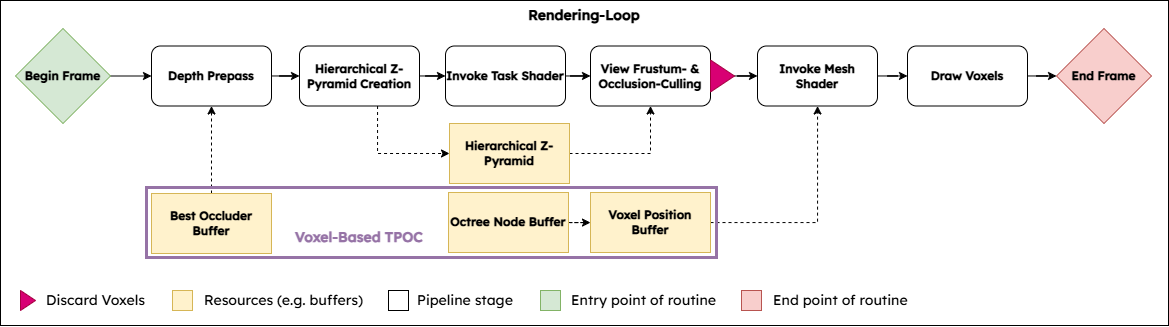
\includegraphics[width=\linewidth]{images/pipeline-rendering-loop.png}
    \caption{The rendering loop and its resources.}
    \label{fig:rendering-loop}
\end{figure*}

\subsection{Sparse Voxel Octree}

\noindent
Our approach uses a point cloud generated by voxelizing triangle meshes based on the work of \cite{b5}. 
The point cloud is stored as a position list, consumable by the \ac{GPU}. A second data structure is 
necessary for spatial computation, so voxels can be efficiently approximated by larger geometry. 
We chose a custom \ac{SVO} implementation that can easily be transferred to the \ac{GPU}. \\

\noindent
The data structures are bound to the \ac{GPU} pipeline and can be updated as needed. Updating the scene data 
involves updating the voxel list and recomputing the best occluders. Recurring real-time updates to the 
scene were not part of our measurements.

\subsection{Hierarchical Z-Buffering}

\noindent
In the past, the \ac{HZB} algorithm has been slightly adapted for use on the \ac{GPU}. During the rendering 
routine, a small set of best occluders is drawn to the depth buffer during a depth prepass, without invoking 
the pixel shader. This depth information is subsequently converted into a \ac{HZB} pyramid, which is a mip 
map chain containing the depth information for increasingly large parts of the screen space per texel. \\


\subsection{Mesh Shading}

\noindent
Although \ac{TPOC} is generally compatible with traditional rendering pipelines, we choose the 
\ac{GPU}-driven mesh shading pipeline for computing large amounts of voxels. Compared to the use 
of geometry shaders or instancing, mesh shading promises the best performance for large amount 
of on-chip created voxels, while also being compatible with modern \ac{GPU}-based rendering and 
culling algorithms. \\ % @TODO: Source for mesh shading

\noindent
We used the mesh shading pipeline (\ac{TPOC-PM}) to evaluate the performance and efficiency of 
\ac{TPOC} in this new context of voxel rendering as compared to the more traditional culling of 
individual octree nodes (\ac{TPOC-PON}). 

\subsection{Generating Best Occluders} \label{sec-gen-best-occluders}

\noindent
Traditionally, the best occluders are artist-authored meshes, which are expected to be occluding a lot 
of small instances during runtime. This can, for example, be a house, a large wall, or similar large 
geometry. Rendering them during a depth prepass enables the occlusion of smaller mesh instances. \\

\noindent
In voxel rendering, this is not applicable as is, since the individual meshes, i.e., the voxels, are all 
of uniform size. Additionally, the best occluders might need to be altered during runtime, since 
volumetric voxel representations often allow run-time manipulation of the voxel data. A predetermination 
of the best occluders is thus not possible as it is for static, non-voxel triangle meshes. \\

\noindent   % @TODO: Check sentence "even though the measurements did not include ..."
We have implemented a dynamic way of selecting the best occluder geometry for the depth prepass, even 
though the measurements did not include a runtime alternation of the voxel data. To select appropriate 
occluders, a buffer of octree nodes is used, which contains a list of the best occluders within the scene. \\

\noindent
To compute a best occluder, the property of a full node is recursively propagated upwards within the hierarchy, 
so the largest possible octree node, which is completely filled with voxels is used as an approximation for 
all the contained voxels. All best occluder nodes are then added to a buffer that can be sent to the \ac{GPU} for 
use in the depth prepass. \\

\noindent
Ultimately, the best occluders exchange a large amount of voxels with larger, octree node-sized boxes for 
computing the depth prepass. This way, drawing geometry to approximate the volume of the voxel scene is 
more efficient because of the reduced number of meshes contributing to the prepass. 
Fig.~\ref{fig:best-occluder-selection} shows a visualization featuring the best occluders in relation 
to the final voxel scene. Because of \ac{TPOC}, the number of voxels drawn during the prepass can be reduced 
from about 3 million to only 8256 best occluder voxels.

\begin{figure}
    \centering
    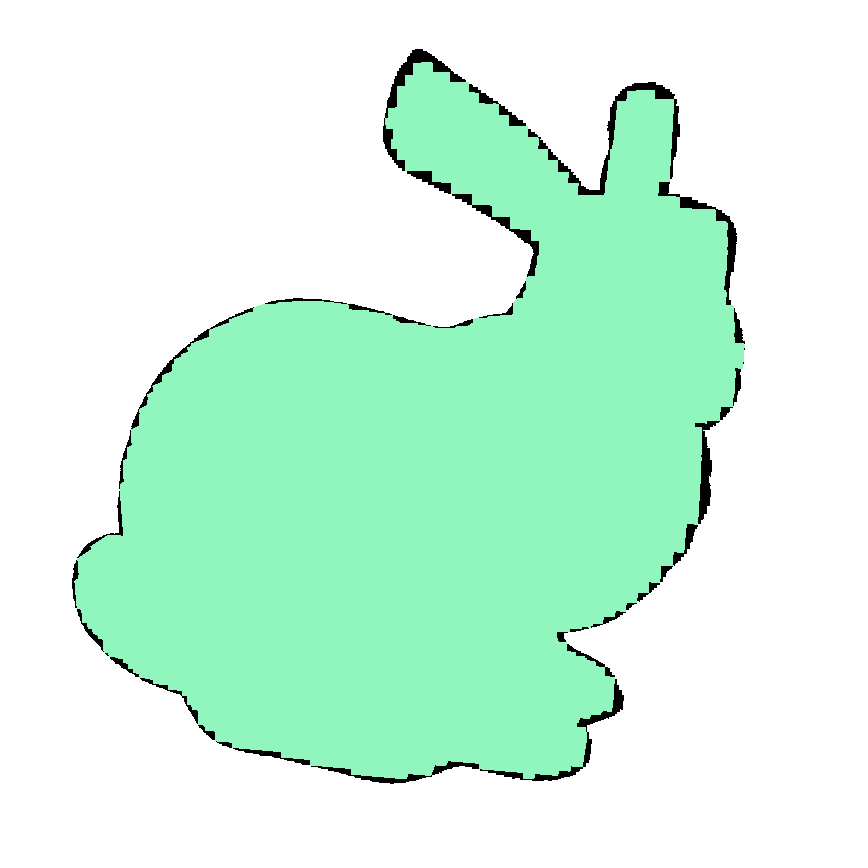
\includegraphics[width=150px]{images/bunny-best-occluder-outline.png}
    \caption{The bunny model silhouette in black and the best occluders selected for the prepass in green.
    Because of \ac{TPOC}, only 8256 best occluders need to be drawn to approximate the scene's volume instead of about 3 million voxels.}
    \label{fig:best-occluder-selection}
\end{figure}

\subsection{Depth Prepass} \label{sec-depth-prepass}

\noindent
The frame's computation starts by computing the depth prepass, which is the custom
render pass central to the occlusion culling. In this pass, a compute shader is invoked
that takes the best occluders and draws them to the depth buffer. This depth pass does
not draw to the back buffer, making the computation relatively efficient. \\

\noindent
After the depth buffer is created, it is used to create a mip map chain containing the depth 
data from the depth buffer, the \ac{HZB} pyramid. To create the mip map chain, the full-resolution 
depth buffer is processed by a compute shader, which calculates the farthest depth value out 
of four texels and outputs it to the next higher mip level. The resulting mip map chain consequently 
contains a coverage of differently sized screen-space quads with the respective farthest depth 
value. The mip map chain is subsequently used in the task shader (amplification shader) during the 
occlusion culling. Fig.~\ref{fig:hzb-pyramid-viz} shows an exemplary \ac{HZB} pyramid.

\begin{figure}
    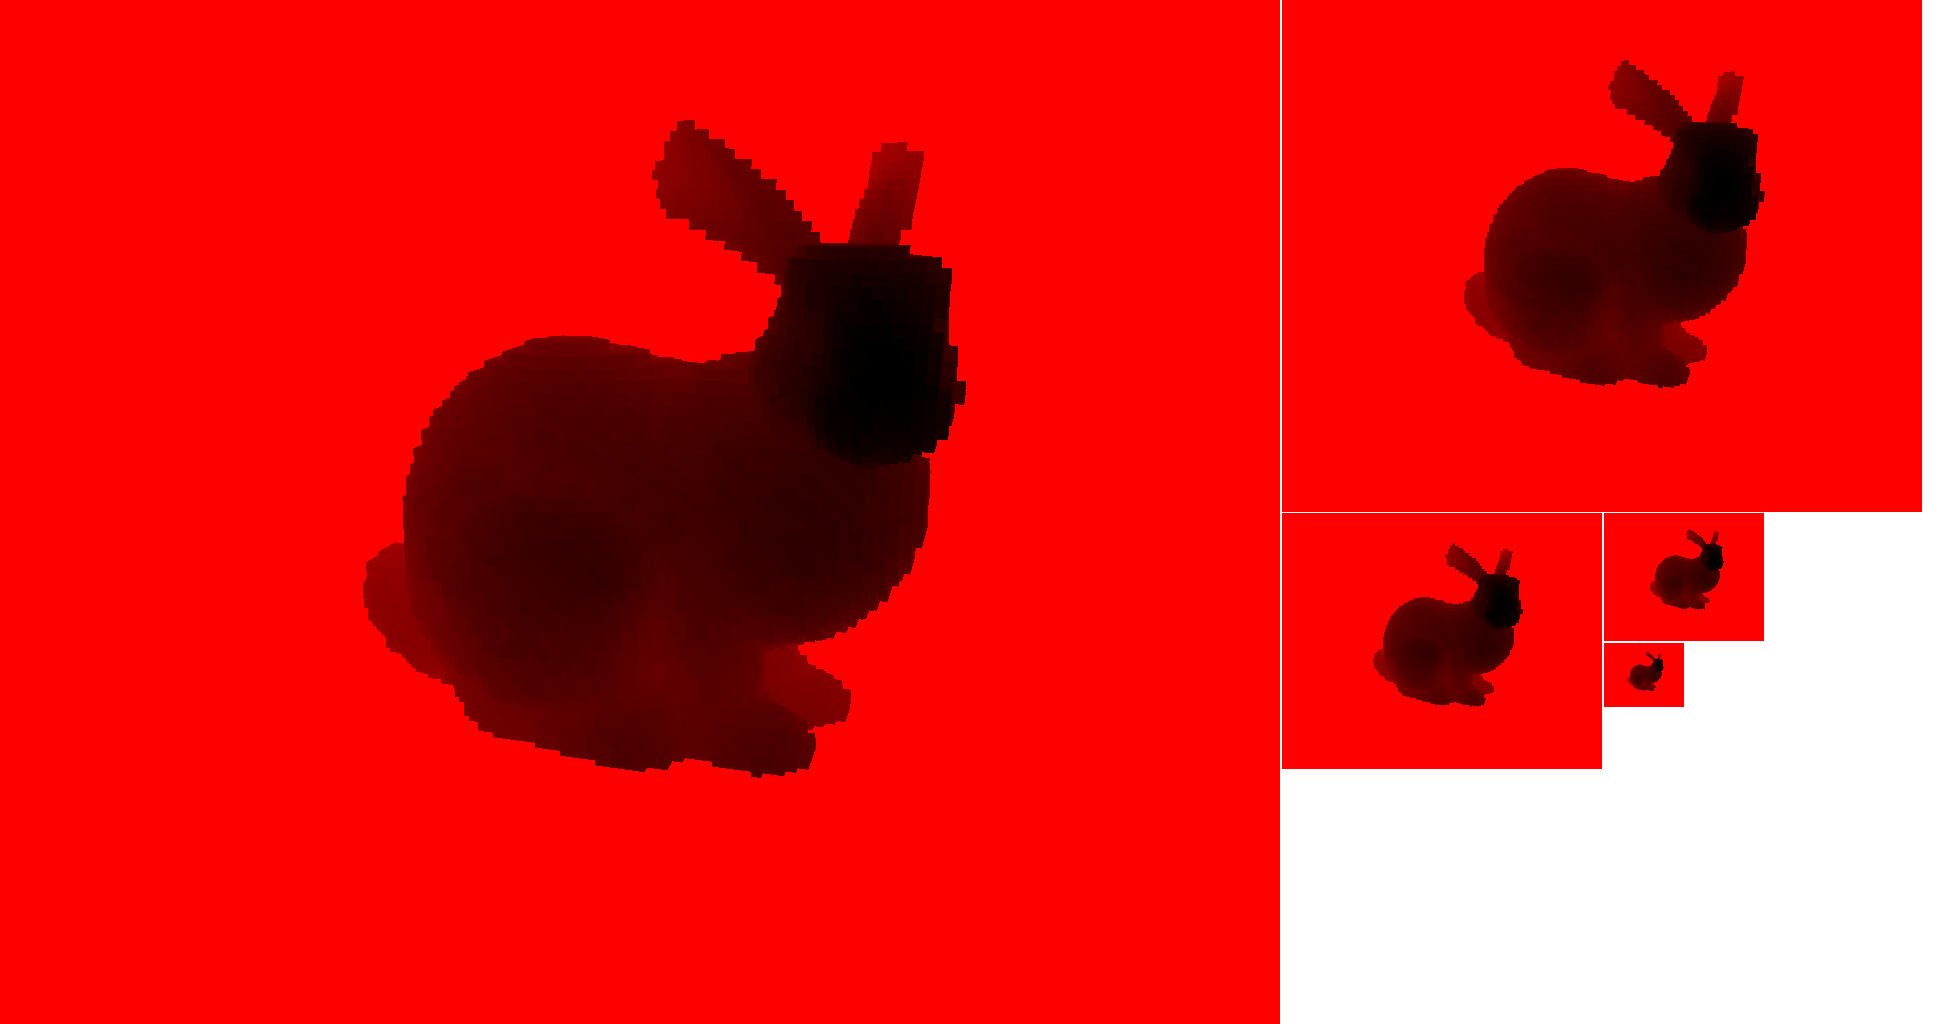
\includegraphics[width=\linewidth]{images/hiz-pyramid.png}
    \caption{The \ac{HZB} pyramid of the \emph{Bunny} scene.}
    \label{fig:hzb-pyramid-viz}
\end{figure}

\subsection{Occlusion Culling} \label{sec-occlusion-culling}

\noindent
For the main rendering pass, we propose generating the voxels directly on the \ac{GPU}, since this 
guarantuees fast processing of geometry and allows to create meshlets without precomputation.
Consequently, our implementation treats each voxel as one meshlet. \\

\noindent
When the voxels are scheduled for final rendering, the task shader precomputes the point cloud 
and only dispatches the voxels for a final draw if they are not found to be occluded. The occlusion 
culling is implemented similarly to other comparable approaches. First, bounding boxes are created 
around each point of the point cloud, which are then projected to screen space. After that, 
a two-dimensional screen-space rectangle is constructed around the bounding box using the minimum 
and maximum values on the \emph{y} and \emph{z} axes. Additionally, the minimum \emph{z} value of 
the bounding box is computed and stored alongside the \emph{y} and \emph{z} values. Using these 
coordinates, the four corners of the bounding boxes are sampled from the \ac{HZB} pyramid, and the 
resulting depth values are compared against the minimum \emph{z} value. If either of the 
\ac{HZB} pyramid samples is further away from the camera than the minimum \emph{z} value, the current 
voxel might be completely or partially visible. Conversely, as long as all samples are nearer to 
the camera than the minimum \emph{z} value, the voxel can safely be assumed to be occluded. This 
sampling starts using the highest mip level and continues down the mip map chain until the voxel is 
found to be fully occluded or until the hierarchy is fully traversed and the voxel is found to be 
visible. The complete rendering loop is shown in Fig.~\ref{fig:rendering-loop}.

\section{Evaluation} \label{sec-evaluation}

\begin{figure*}
    \begin{subfigure}{100px}
        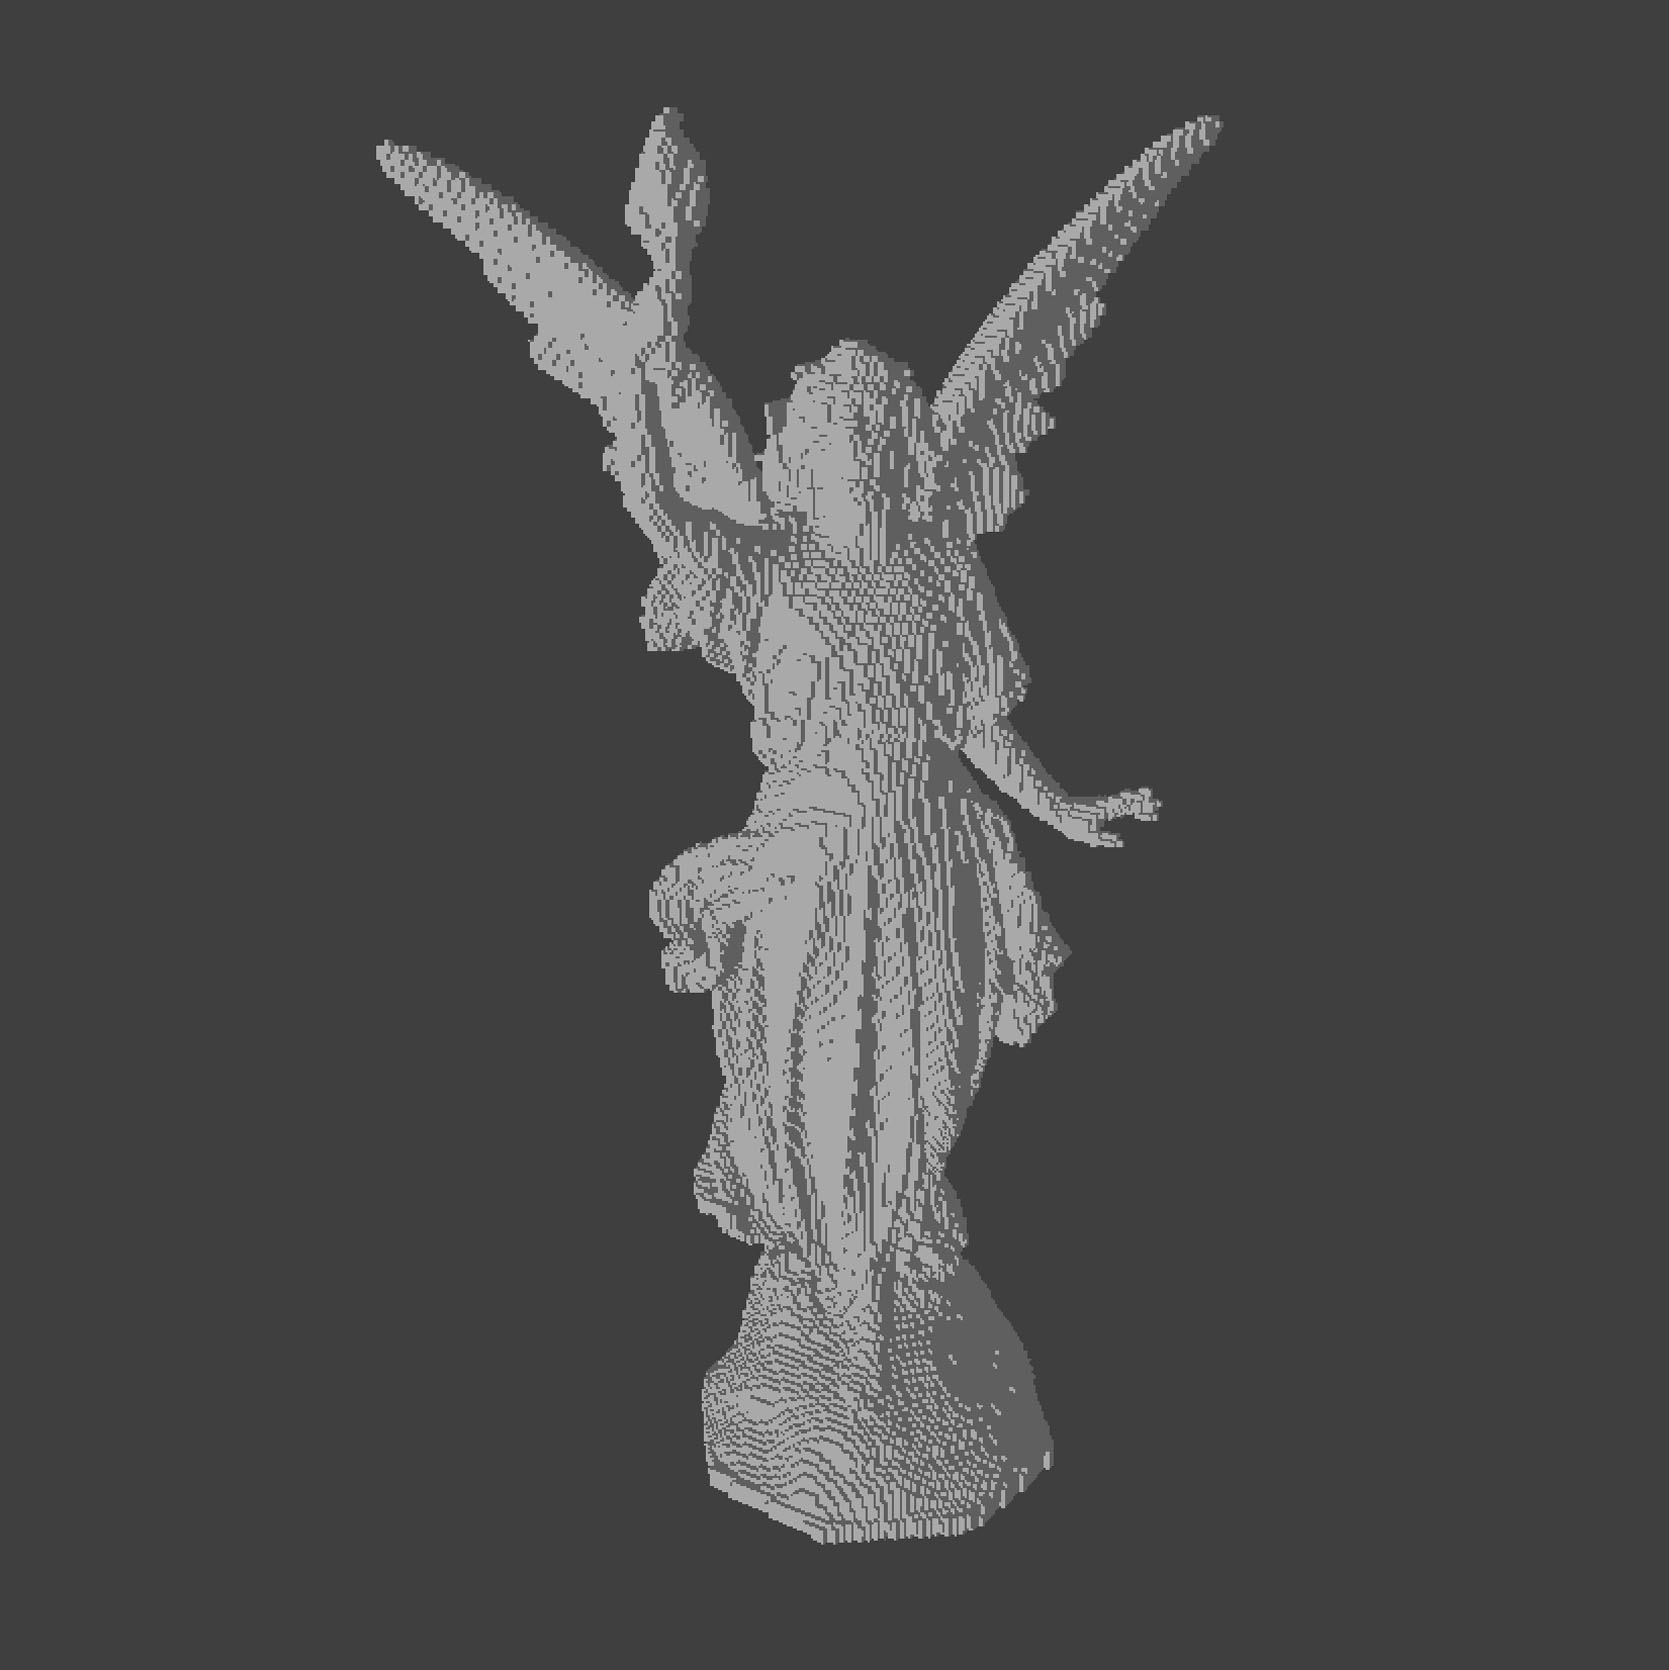
\includegraphics[width=100px]{images/model-lucy.jpg}
        \caption{Lucy \cite{b7}}
        \parbox{\linewidth}{\centering\footnotesize 331,254 voxels,\\ 1600 best occluders}
    \end{subfigure}
    \begin{subfigure}{100px}
        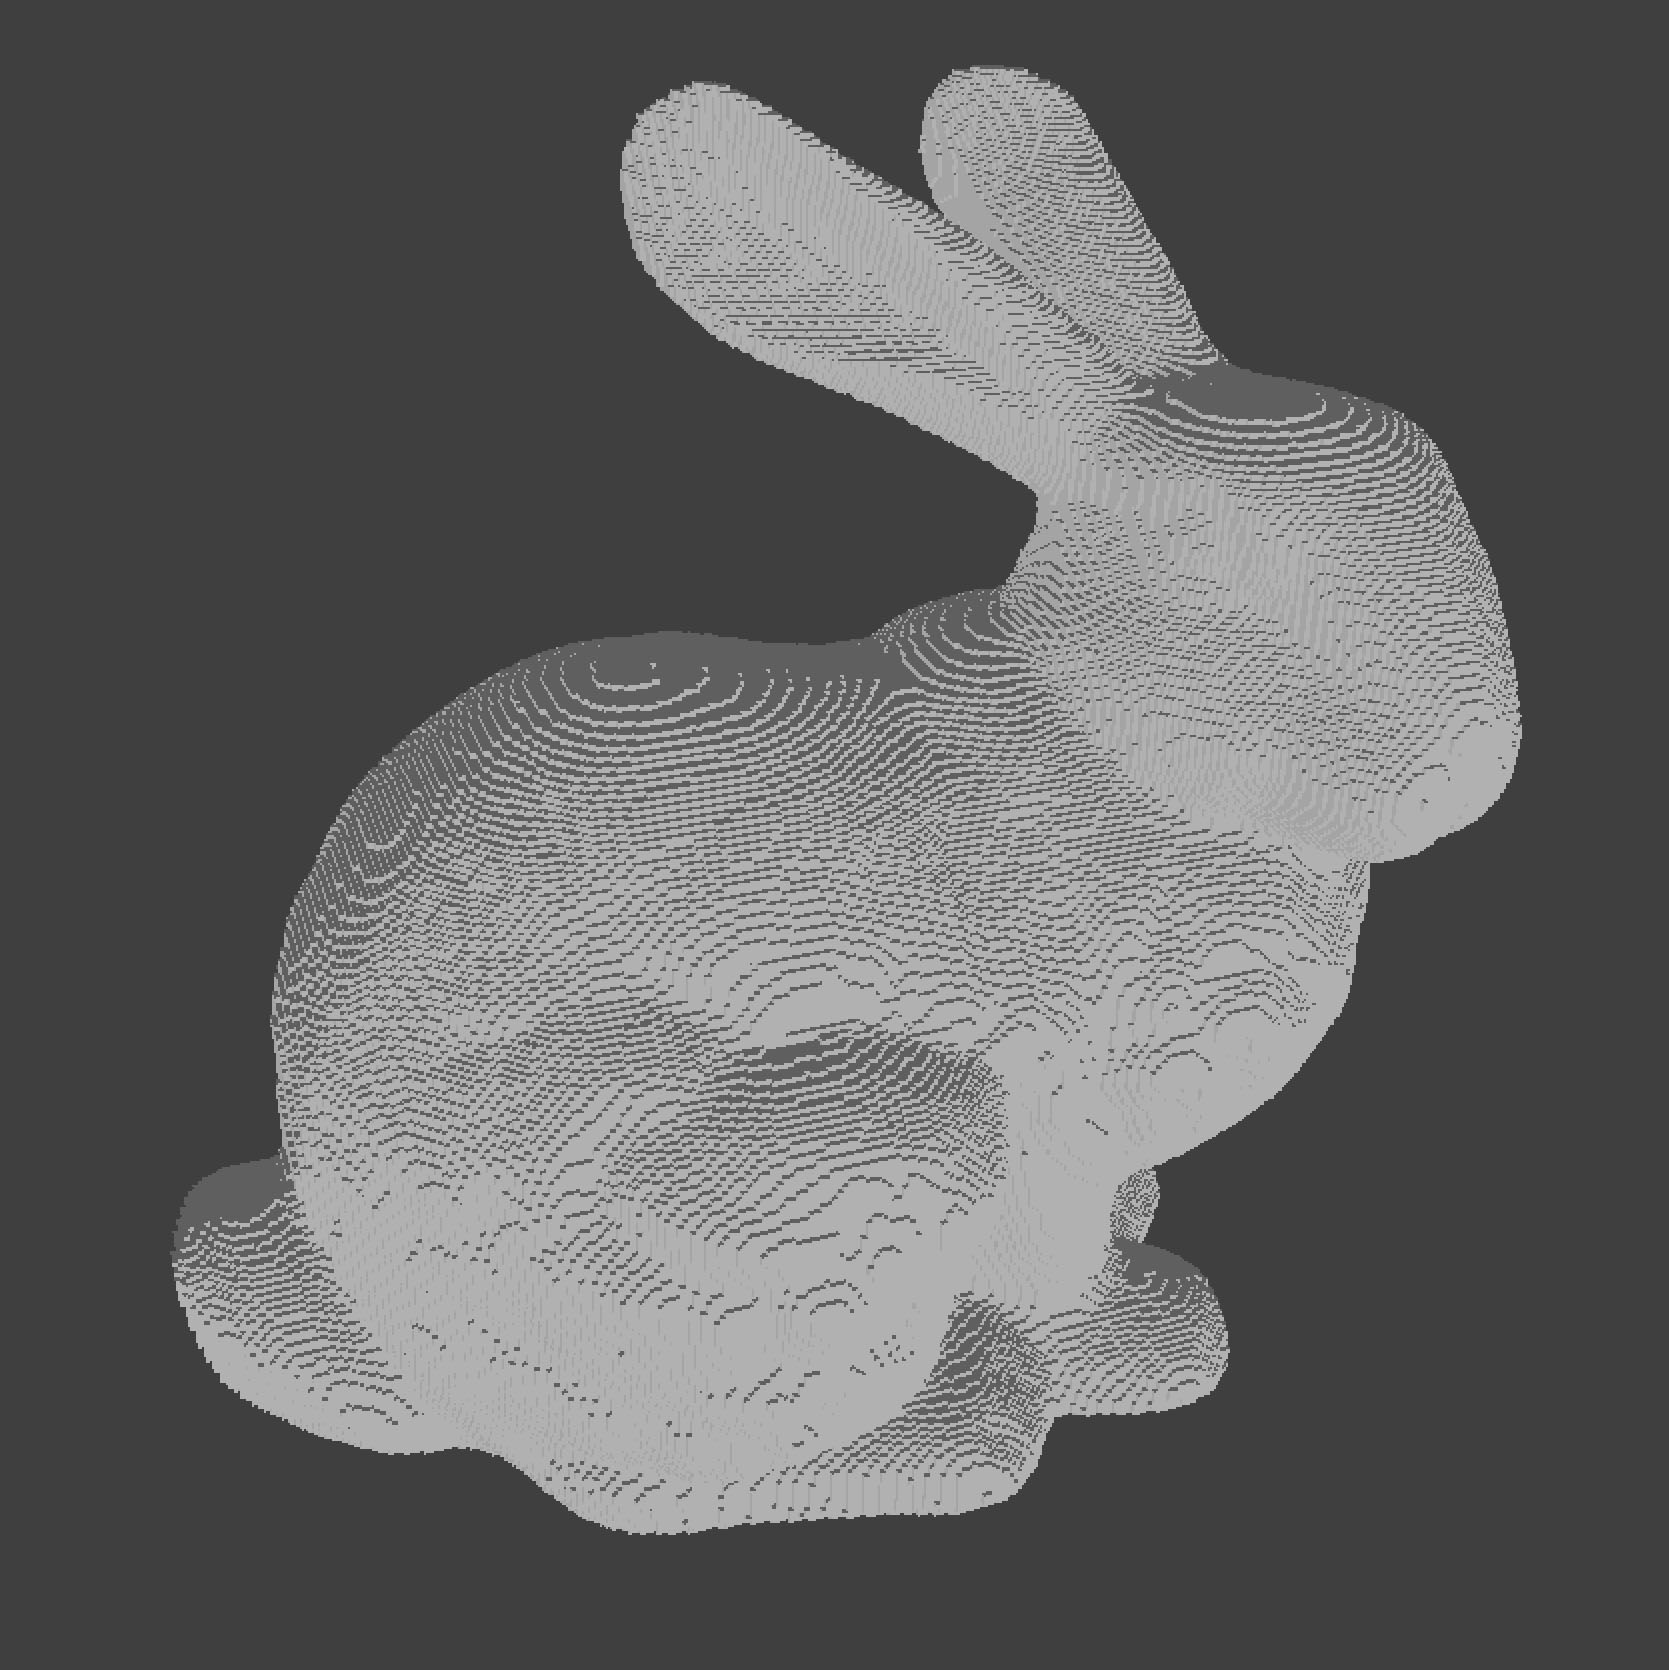
\includegraphics[width=100px]{images/model-bunny.jpg}
        \caption{Stanford Bunny \cite{b7}}
        \parbox{\linewidth}{\centering\footnotesize 3,379,738 voxels,\\ 8256 best occluders}
    \end{subfigure}
    \begin{subfigure}{100px}
        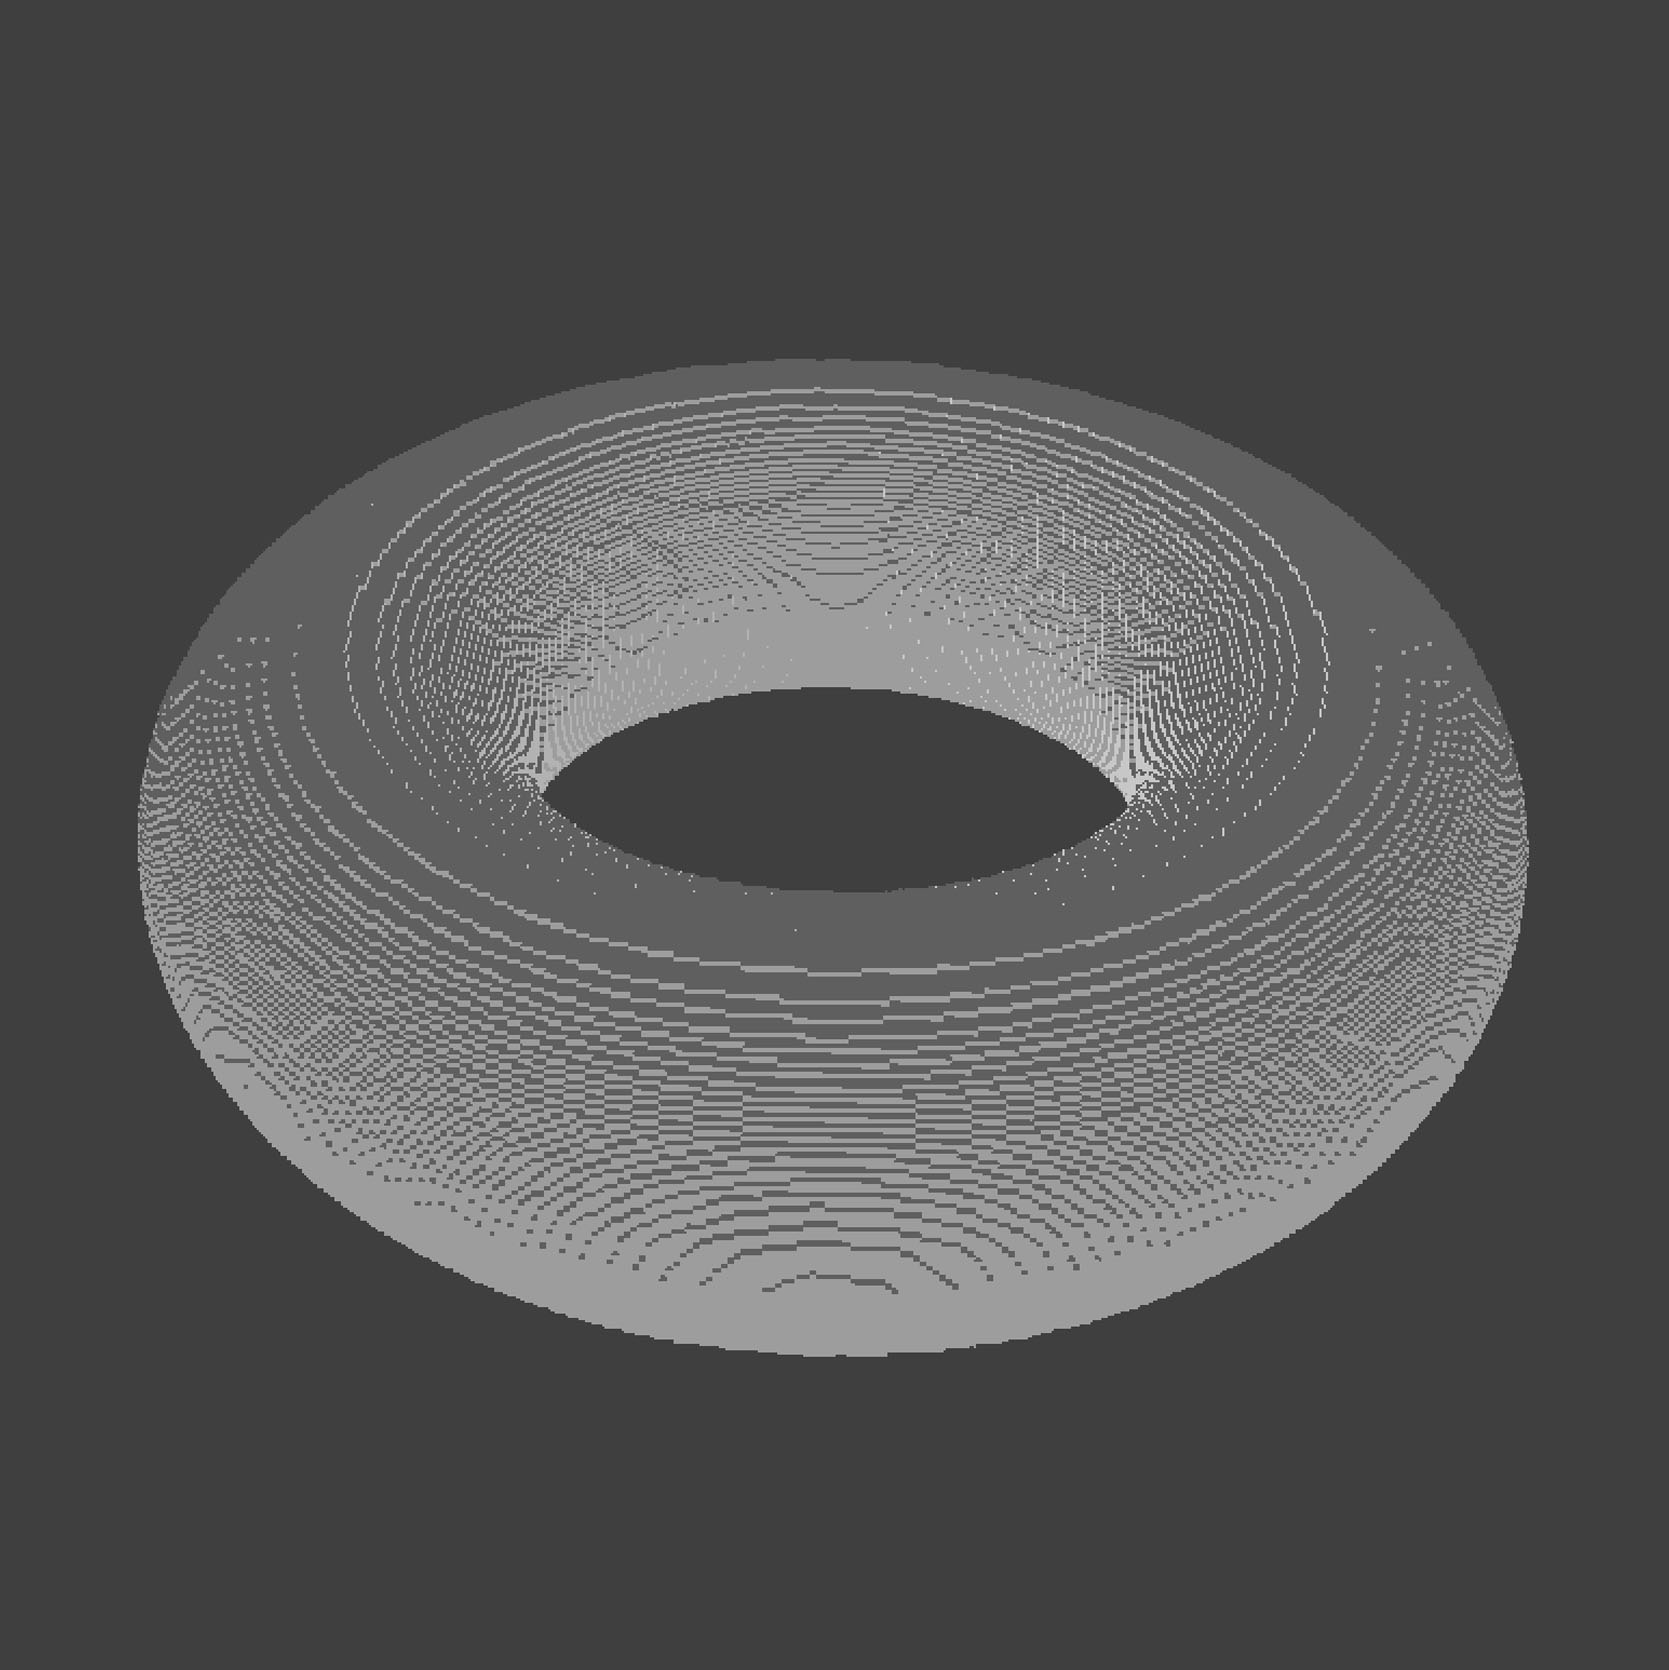
\includegraphics[width=100px]{images/model-torus.jpg}
        \caption{Torus}
        \parbox{\linewidth}{\centering\footnotesize 2,311,006 voxels,\\ 7168 best occluders}
    \end{subfigure}
    \begin{subfigure}{100px}
        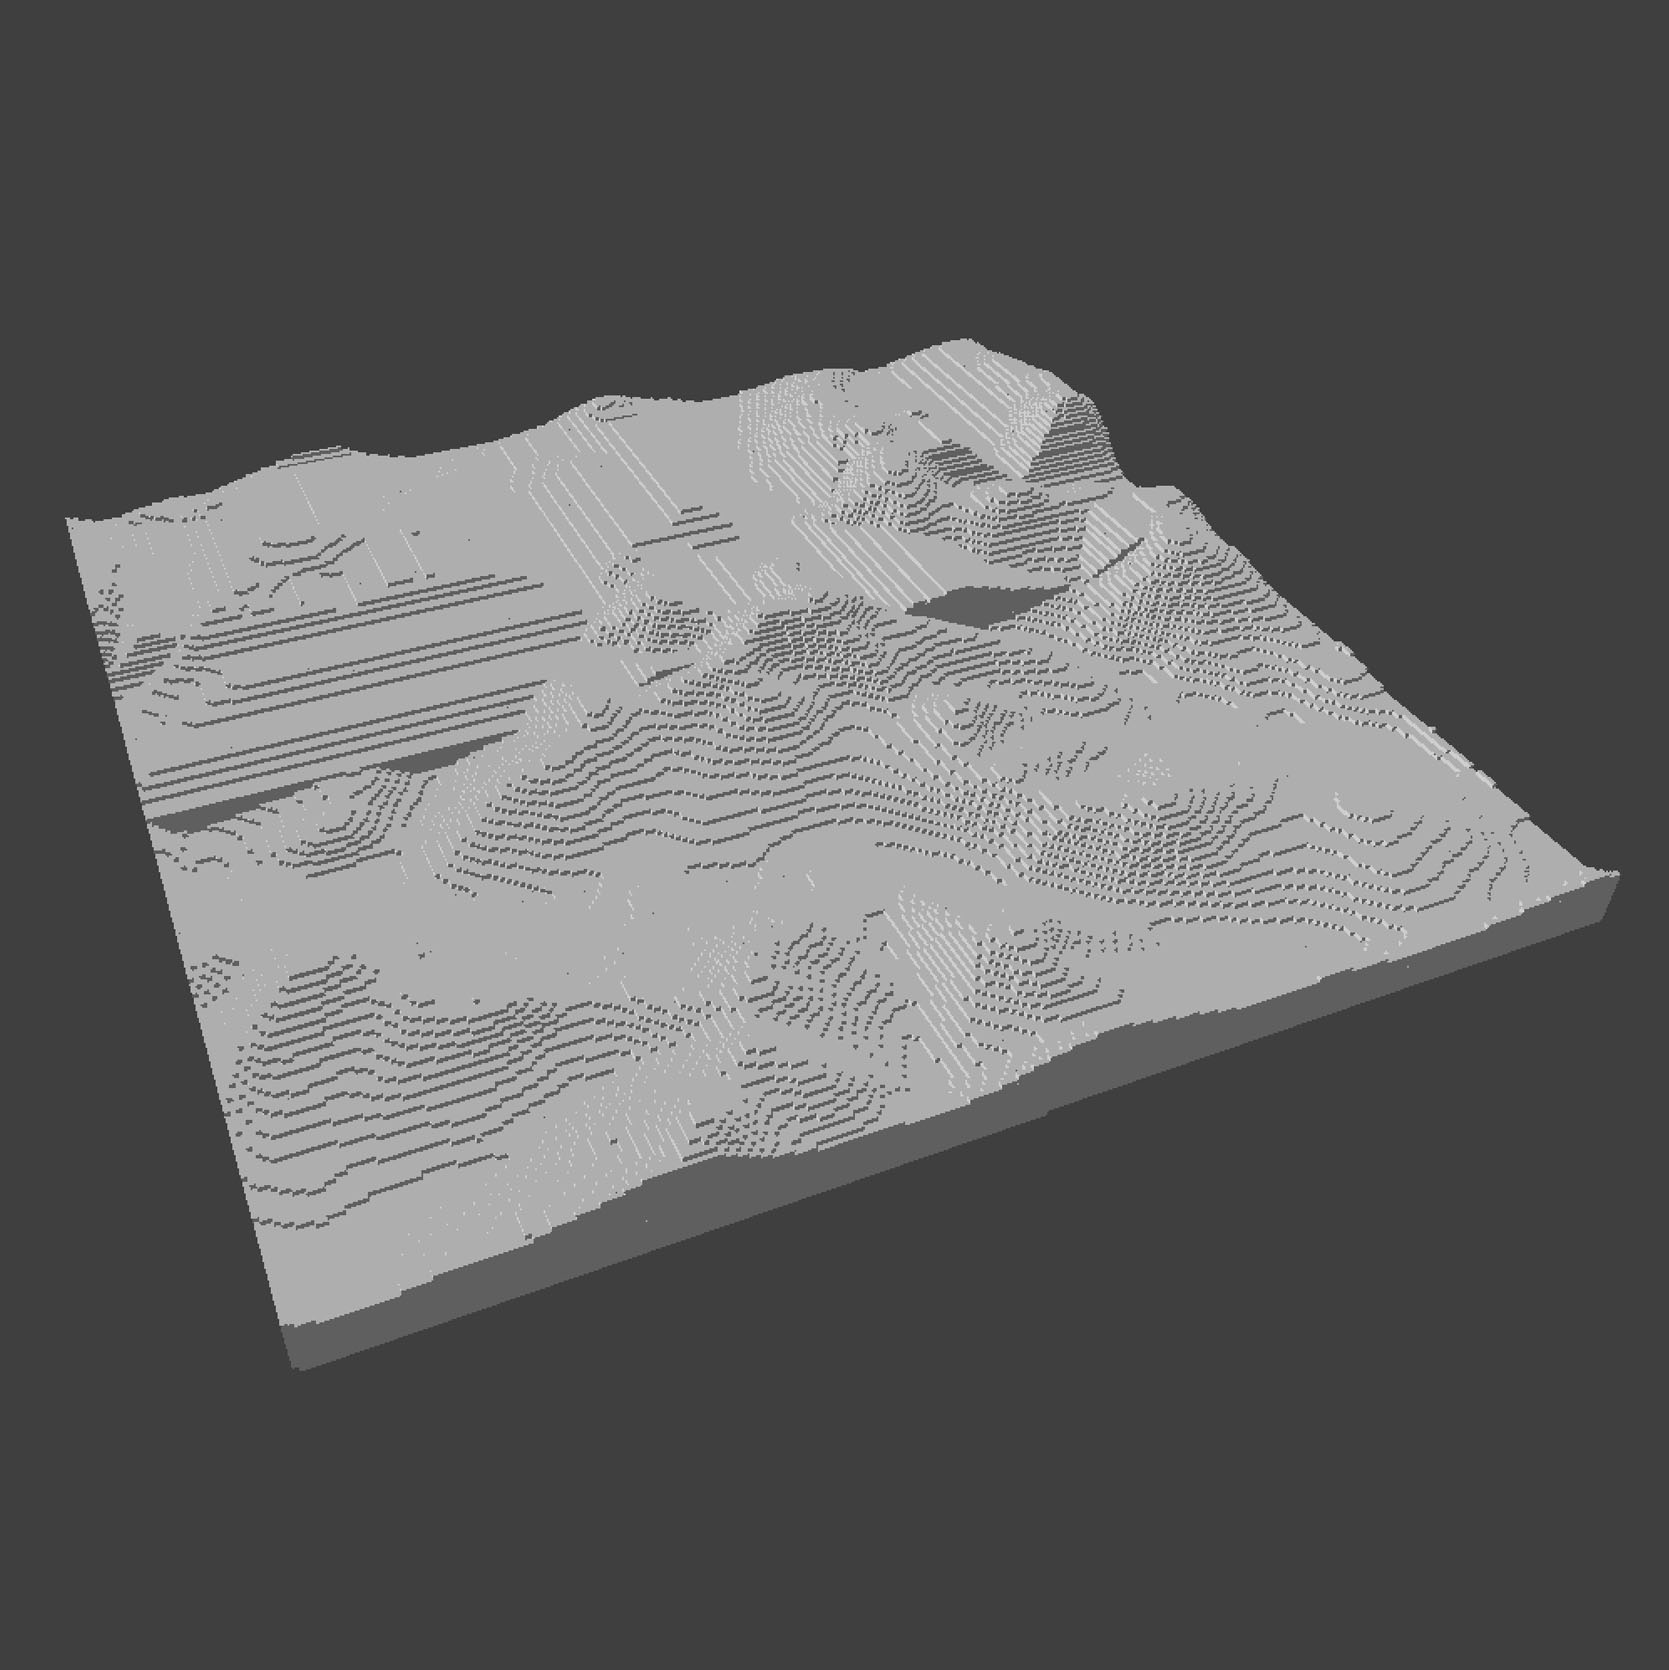
\includegraphics[width=100px]{images/model-terrain.jpg}
        \caption{Terrain}
        \parbox{\linewidth}{\centering\footnotesize 953,362 voxels,\\ 6976 best occluders}
    \end{subfigure}
    \begin{subfigure}{100px}
        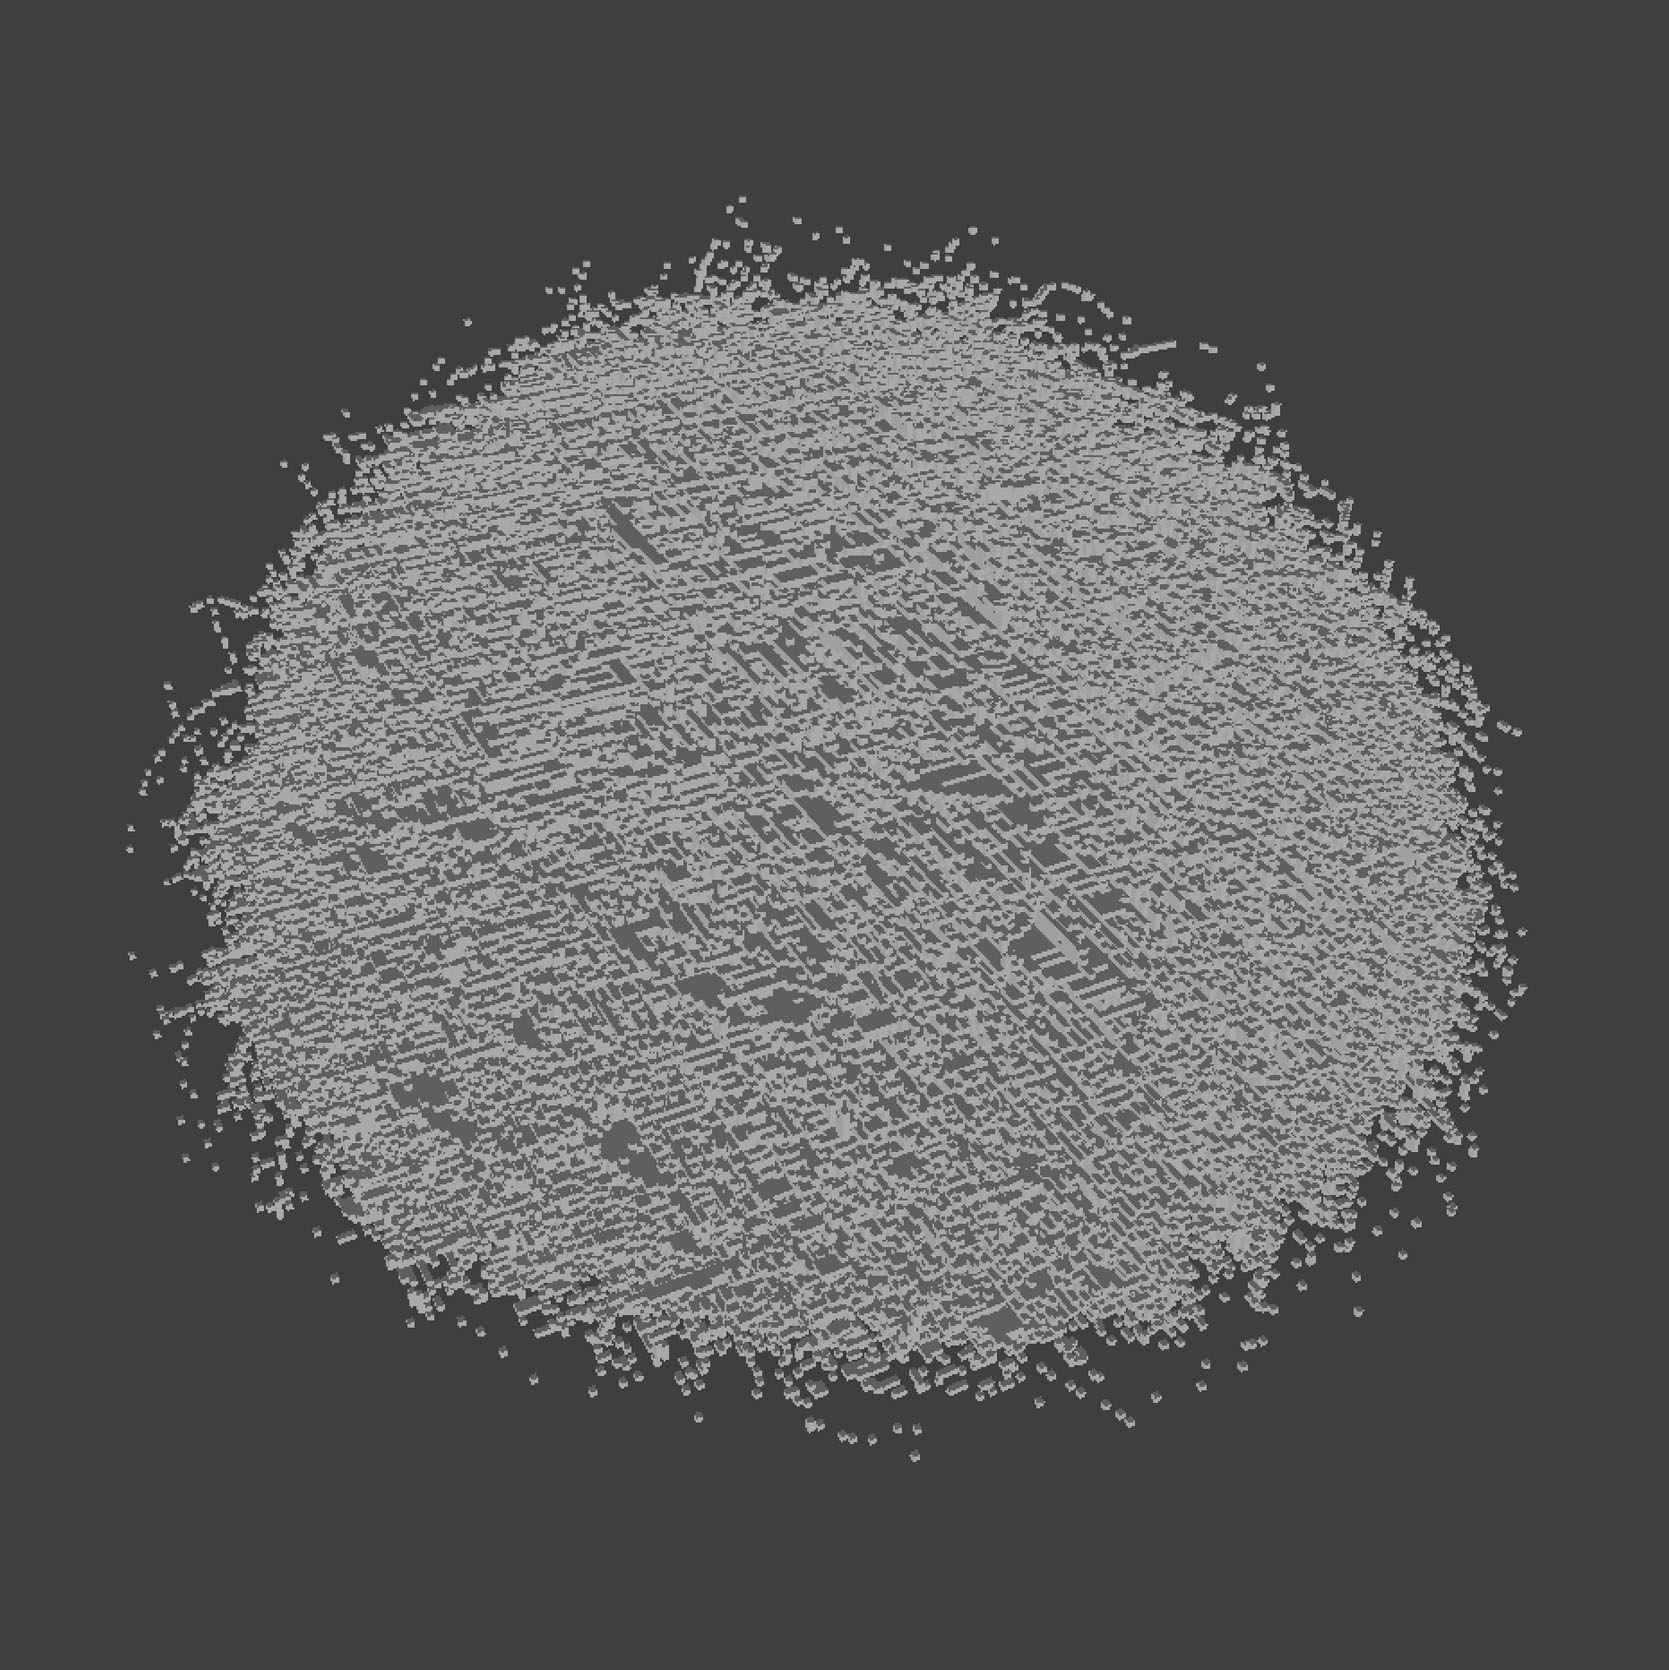
\includegraphics[width=100px]{images/model-hairball.jpg}
        \caption{Hairball \cite{b8}}
        \parbox{\linewidth}{\centering\footnotesize 1,652,435 voxels,\\ 5056 best occluders}
    \end{subfigure}
    
    \caption{The scenes used for the experimental evaluation of the algorithm.}
    \label{fig:models}
\end{figure*}

\noindent
We evaluated the two occlusion culling configurations \ac{TPOC-PON} and \ac{TPOC-PM} with respect to culling 
efficiency, \ac{CPU} runtime performance, \ac{GPU} runtime performance, and pixel overdraw. We used five 
test scenes featuring different geometrical characteristics, shown in Fig.~\ref{fig:models}. The tests were 
executed on a Windows 10 system with an AMD Ryzen 9 9950X and a NVIDIA GeForce RTX 4090, using Shader Model 
6.7 and a fixed resolution of $1280 \times 900$. All tests were performed using a unified camera animation in 
order to consider a variety of camera angles and provide more meaningful results in repsect to real use-cases. 
During the animation, the camera follows an orbital path around the scene, while also moving up and down again. 
This method ensures a balanced representation of the scene's topological characteristics.


\subsection{Best Occluder Selection} \label{subsec-best-occluder-selection}

\noindent
The time spent on querying the best occluders within the octree is relevant for dynamically updating 
voxel data in real time. It is in general dependent on two main factors: the amount of octree nodes 
and the scene's spatial characteristics. \\

\noindent
The more nodes there are, the longer it typically takes to compute the best occluders, as the tree 
hierarchy becomes larger. However, in large scenes without gaps, this scaling effect is mitigated 
by the depth of the tree traversal. In this case the query can exit a subbranch of the octree 
earlier because a larger octree node might already approximate a large part of the volume sufficiently. \\

\noindent
The time measured for the best occluder selection is listed in table \ref{tab:best-occluder-query}. 
All measured scenes had a dimension of $256^3$.

\begin{table}[htbp]
    \begin{center}
        \begin{tabular}{|c|c|c|c|}
            \hline
            \textbf{}&\multicolumn{3}{|c|}{\textbf{Best Occluder Selection - $256^3$}} \\
            \cline{2-4} 
            \textbf{Scene} & \textbf{\textit{Voxel Count}}& \textbf{\textit{Best Occluder Count}}& \textbf{\textit{Time (ms)}} \\
            \hline
            Lucy        & 331,254   & 1600 & 0.317 \\
            Bunny       & 3,379,738 & 8256 & 3.752 \\
            Torus       & 2,311,006 & 7168 & 2.681 \\
            Terrain     & 953,362   & 6976 & 1.267 \\
            Hairball    & 1,652,435 & 5056 & 2.377 \\
            \hline
        \end{tabular}
    \end{center}
    \caption{Measurements of best occluder query.}
    \label{tab:best-occluder-query}
\end{table}

\noindent
In general, the measurements show that the computation time for the best occluders corelates with the voxel count.
However, the topological characteristics of the scenes have to be taken into consideration as well. This is 
indicated by the \emph{Hairball} scene, which compared to its high voxel count has fewer best occluders than 
expected, but takes more time to compute than the \emph{Terrain} scene with more best occluders. \\

\noindent
The results suggest that the query can be used in realtime applications, as most of the measurements stay 
within reasonable time budgets for computation, if 16.6 ms is used as a reference time for one frame. However, 
the measurements were executed on a single thread, and the computation was not optimized thoroughly. The 
duration is expected to be minimized further by chunking the data to limit the size and the amount of octree 
nodes, as well as by applying multi-threaded computations, e.g., computing each chunk in parallel on the \ac{CPU}.

\subsection{Culling Efficiency} \label{subsec-culling-efficiency}

\noindent
Table \ref{tab:culling-efficiency} shows the average culling efficiency for each tested scene measured using 
various camera angles. The table indicates an overall better culling performance when using the \ac{TPOC-PM} 
occlusion culling as compared to the \ac{TPOC-PON} configuration.

\begin{table}[htbp]
    \begin{center}
        \begin{tabular}{|c|cc|cc|}
            \hline
            \textbf{}&\multicolumn{4}{|c|}{\textbf{Avg. Culled Voxels - $256^3$}} \\
            \cline{2-5} 
            \textbf{Scene} & \textbf{\textit{\ac{TPOC-PON}}} & \textbf{\textit{Ratio}} & \textbf{\textit{\ac{TPOC-PM}}} & \textbf{\textit{Ratio}} \\
            \hline
            Lucy        &  190,412      & $57.5 \%$    & 247,226        & $74.6 \%$     \\
            Bunny       &  2,994,528    & $88.6 \%$    & 3,199,472      & $94.7 \%$     \\
            Torus       &  1,951,693    & $84.5 \%$    & 2,140,234      & $92.6 \%$     \\
            Terrain     &  557,134      & $58.4 \%$    & 772,922        & $81.1 \%$     \\
            Hairball    &  954,886      & $57.8 \%$    & 1,070,722      & $64.8 \%$     \\
            \hline
        \end{tabular}
    \end{center}
    \caption{Culling efficiency for each of the tested scenes. The average amount was measured using a 
    unified camera animation to take different camera angles into account. Higher is better.}
    \label{tab:culling-efficiency}
\end{table}

\noindent
The \ac{TPOC-PM} configuration culled an average of $12.2 \%$ more voxels and always resulted in fewer 
voxels computed by the rasterizer and the pixel shader. The measurements also suggest that larger scenes 
with more voxels lead to a higher culling efficiency. This seems plausible, as a higher voxel number 
tends to result in a higher number of best occluders for a static amount of voxels per octree node. As 
the \emph{Hairball} scene shows, \ac{TPOC} works in favor of large, dense geometry and is challenged by 
smaller details, large empty spaces, and holes.

\subsection{CPU Performance} \label{subsec-cou-performance}

\noindent
The average \ac{CPU} time over the course of the unified test animation using \ac{TPOC} is shown in 
table~\ref{tab:cpu-performance}. It was measured for each culling configuration to evaluate the difference 
in runtime performance for the Render-Thread functions of the application. The table shows that the average 
\ac{CPU} performance does not change significantly between the different culling configurations. The small 
changes that are visible in measurements are attributed to the \ac{GPU} performance differences presented 
below. Because of the \ac{GPU}-driven nature of \ac{TPOC}, which results in a low memory bandwidth between 
\ac{CPU} and \ac{GPU}, these changes are rather small. Most of the work is executed on the \ac{GPU} and the 
\ac{CPU} implementations do not change considerably between the \ac{TPOC-PON} and the \ac{TPOC-PM} 
configuration. \\

\begin{table}[htbp]
    \begin{center}
    \begin{tabular}{|c|c|c|c|}
        \hline
        \textbf{}&\multicolumn{3}{|c|}{\textbf{Avg. \ac{CPU} Performance - $256^3$}} \\
        \cline{2-4} 
        \textbf{Thread} & \textbf{\textit{No Culling (ms)}} & \textbf{\textit{\ac{TPOC-PON} (ms)}} & \textbf{\textit{\ac{TPOC-PM} (ms)}}  \\
        \hline
        Render-Thread      &  0.1165   & 0.1135    &  0.1122   \\
        \hline
    \end{tabular}
\end{center}
\caption{Average \ac{CPU} performance using different occlusion culling configurations.}
\label{tab:cpu-performance}
\end{table}

\subsection{GPU Performance} \label{subsec-gpu-performance}

\noindent
The \ac{GPU} performance shown in Fig.~\ref{fig:gpu-performance-full} was measured for each scene and each 
culling configuration. The average measurements indicate a significant performance increase in every scenario. 
The greatest average increase was measured using the \emph{Bunny} scene, which featured a large volume and a 
high number of voxels. Those characteristics seem to work in favor \ac{TPOC}, as a large volume and a high 
voxel count result in an efficient approximation of the given scene. Best occluders can potentially be computed 
more efficiently, since a lot of adjacent octree nodes are expected to be full. \\

\begin{figure}
    \begin{center}
        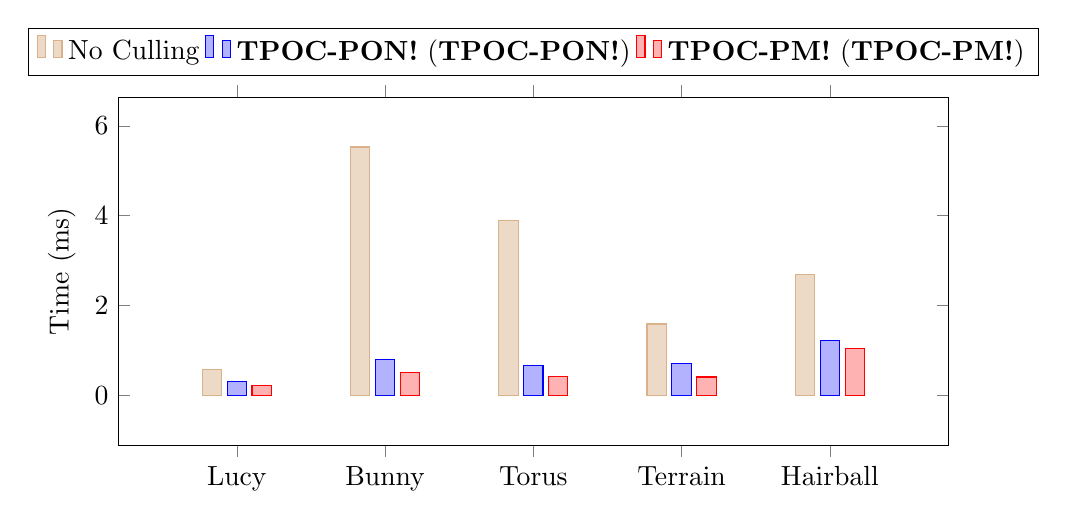
\begin{tikzpicture}
        \begin{axis}
            [height=6cm,
            width=\linewidth,
            x tick label style={/pgf/number format/1000 sep=},
            ylabel={Time (ms)},
            legend style={at={(0.5,1.2)}, anchor=north, legend columns=3},
            symbolic x coords={Lucy, Bunny, Torus, Terrain, Hairball},
            xtick=data,
            ymin=0,
            enlargelimits=0.2,
            ybar,
            bar width=7pt]

            \addplot[brown!60, fill=brown!30] coordinates {(Lucy,0.58) (Bunny,5.53) (Torus,3.90) (Terrain,1.59) (Hairball,2.69)};
            \addplot[blue, fill=blue!30] coordinates {(Lucy,0.32) (Bunny,0.80) (Torus,0.66) (Terrain,0.71) (Hairball,1.22)};
            \addplot[red, fill=red!30] coordinates {(Lucy,0.22) (Bunny,0.51) (Torus,0.42) (Terrain,0.41) (Hairball,1.04)};
            \legend{No Culling, \ac{TPOC-PON}, \ac{TPOC-PM}}
        \end{axis}
        \end{tikzpicture}
    \end{center}
    \caption{The average \ac{GPU} performance measured for each scene, using both the \ac{TPOC-PON} 
    configuration and the \ac{TPOC-PM} configuration.}
    \label{fig:gpu-performance-full}
\end{figure}

\noindent
A closer inspection of the individual pipeline stages revealed that the depth prepass is more or less static in 
computation time for both configurations, as it scales with the screen resolution. This means that the overhead 
of the algorithm scales with screen resolution and the number of the best occluders drawn during the prepass. 
Both tested configurations perform similarly during the depth prepass and both the copy and the generation of the 
\ac{HZB} are roughly constant in this testing scenario. Only the drawing of the best occluders varies significantly 
for different scenes, as the amount of best occluders changes from one scene to another. \\

\noindent
The most significant differences in performance originate from the main draw pass, which includes the task shader, 
the mesh shader, the rasterizer, and the pixel shader. The culling of voxels leads to a lower computational 
load on those pipeline stages, which in turn considerably reduces the overall render time. The data shows that the 
performance gains outweigh the overhead introduced by the occlusion culling in all tested cases.  

\subsection{Overdraw} \label{subsec-overdraw}

\noindent
Analyzing the overdraw for each scene helps to understand where unnecessary pixel shader 
invocations occur. We tested different angles for each scene and recorded overdraw of individual 
pixels using no occlusion culling, the \ac{TPOC-PON}, and the per-meshlet occlusion 
culling configuration. Fig.~\ref{fig:overdraw} shows an exemplary overdraw visualization for the 
\emph{Bunny} scene. \\

\begin{figure}
    \begin{subfigure}{60px}
        
\includegraphics[width=60px]{images/overdraw-bunny2-nocull.png}
        \caption{No Culling}
        \parbox{\linewidth}{\centering\footnotesize }
    \end{subfigure}
    \begin{subfigure}{60px}
        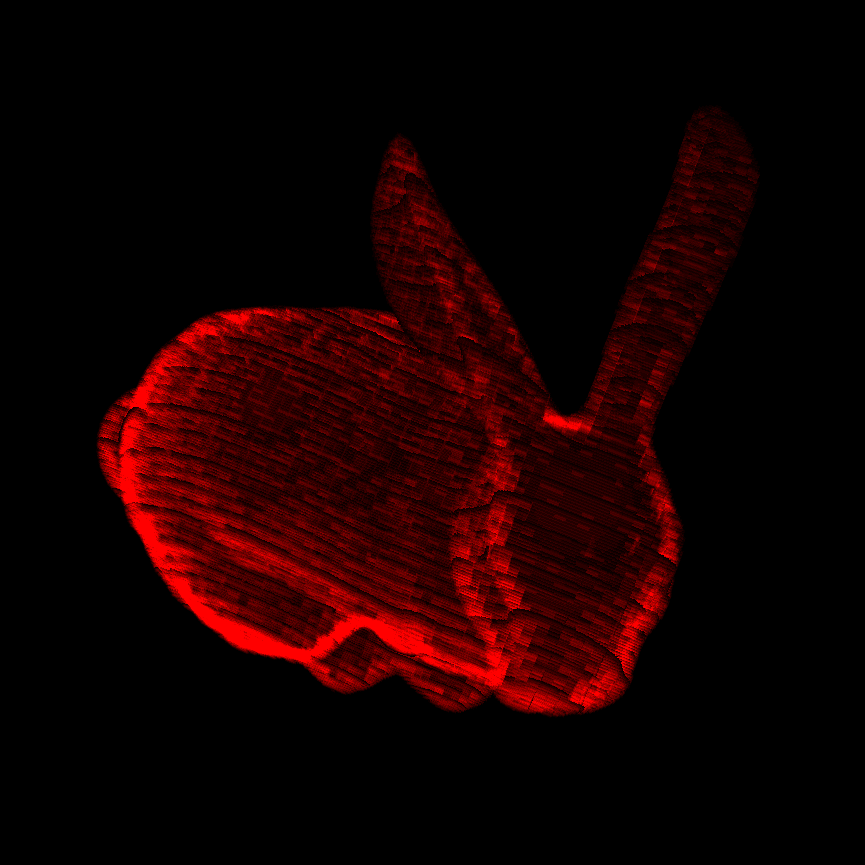
\includegraphics[width=60px]{images/overdraw-bunny2-pooc.png}
        \caption{\ac{TPOC-PON}}
        \parbox{\linewidth}{\centering\footnotesize }
    \end{subfigure}
    \begin{subfigure}{60px}
        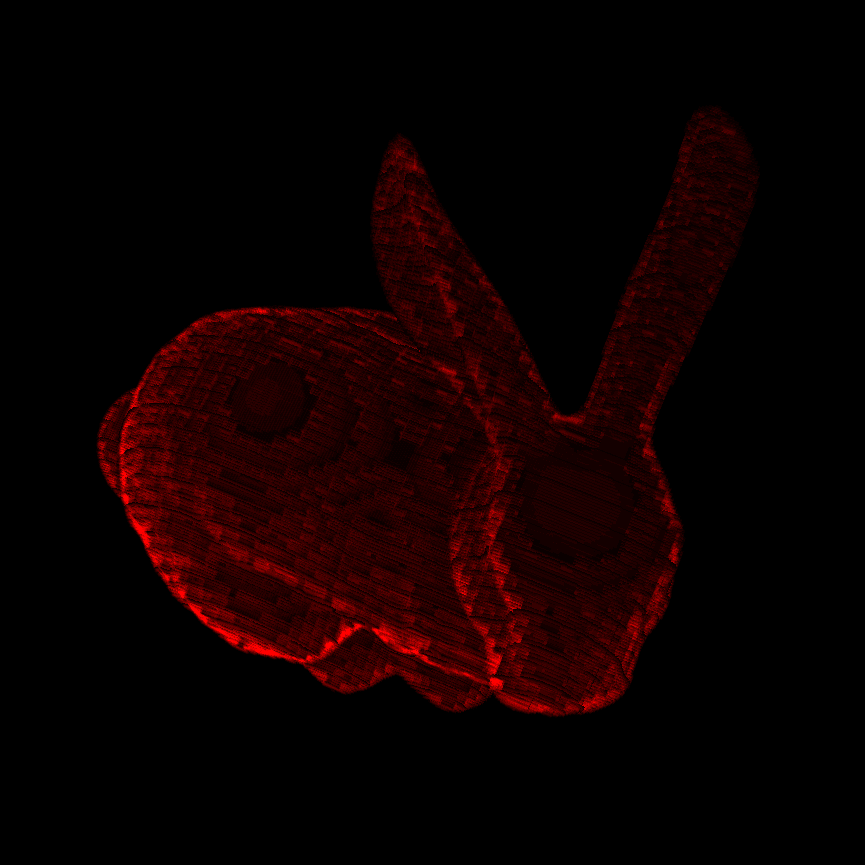
\includegraphics[width=60px]{images/overdraw-bunny2-pmoc.png}
        \caption{\ac{TPOC-PM}}
        \parbox{\linewidth}{\centering\footnotesize }
    \end{subfigure}
    \begin{subfigure}{60px}
        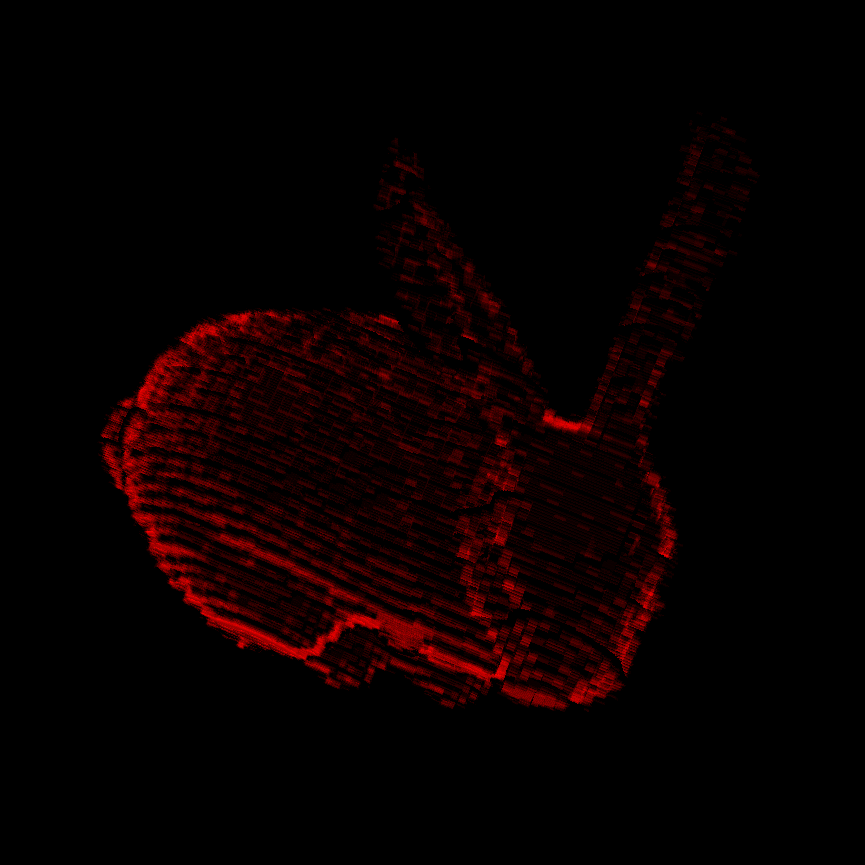
\includegraphics[width=60px]{images/overdraw-bunny2-diff.png}
        \caption{Diff. (b) and (c)}
        \parbox{\linewidth}{\centering\footnotesize }
    \end{subfigure}
    
    \caption{Overdraw visualization for the \emph{Bunny} scene. The values are enhanced for 
    better readability.}
    \label{fig:overdraw}
\end{figure}


\noindent
Image (a) shows that no culling results in a lot of overdraw for some camera angles tested. (b) shows 
the \ac{TPOC-PON}, which features less overdraw overall but still a visible outline 
for the voxels that were not culled by the best occluders. (c) shows the \ac{TPOC-PM} 
configuration, which was able to reduce overdraw considerably as compared to (a) and (b). The outline 
of the scene is smaller and not as heavily overdrawn as the outline in (b), which is attributed to the 
more granular culling of voxels, even within otherwise visible octree nodes. (d) shows the difference 
between (b) and (c), which clearly indicates that the visible surface of the scene can be better 
optimized in terms of overdraw when using \ac{TPOC-PM}. \\

\noindent
Different angles lead to less overdraw and lower differences between all configurations. Nevertheless, 
in all cases the \ac{TPOC-PM} configuration was able to reduce overdraw up to $84 \%$ as compared to 
a pipeline without culling.

\section{Conclusion} \label{sec-conclusion}

\noindent
We have shown that the \ac{HZB} algorithm can be adapted for efficient and dynamic use in rasterized, voxel-based 
volumetric rendering. An approach has been presented that makes use of an octree data structure to approximate 
the scenes invisible voxel data and subsequently uses this data to efficiently draw the best occluders for occlusion 
culling. \\

\noindent
We compared two similar culling configurations within the \ac{HZB} approach and showed that the use of the 
modern mesh shading pipeline considerably increases culling efficiency and, ultimately, overall performance.
The increase in performance compared to the base pipeline without occlusion culling ranged from $61.3 \%$ for 
the \emph{Hairball} scene up to $90.7 \%$ for the \emph{Bunny} scene. The measurements showed that the modern 
mesh shading pipeline allows for a more granular culling of voxels and outperforms the compared per-octree 
node occlusion culling by an average of $29 \%$ in terms of time spent on the \ac{GPU}. \\

\noindent 
Our approach to the \ac{TPOC-PM} implementation can be used to increase performance for suitable scenes by up 
to $90\%$ compared to a pipeline without occlusion culling and by up to $42\%$ compared to \ac{TPOC-PON}, while 
preserving a manageable overhead. In addition, it can be used for dynamically changing scenes since the best 
occluders can be determined during runtime, instead of being manually picked beforehand. \\

\noindent
We conclude that \ac{TPOC} can successfully be applied to high-resolution voxel scenes featuring large, dense 
geometry. In contrast, scenes featuring fine, thin details, holes, or large areas without any geometry are 
generally challenging for the algorithm.

\section{Future Work} \label{sec-future-work}

\noindent
The dynamic update needs to be tested thoroughly to evaluate the capability of the algorithm to handle updating 
larger scenes while also providing reasonable budget for other \ac{CPU} operations. The determination of the best 
occluders could potentially be optimized further by introducing multi-threading. One approach might be to 
compute the best occluders for the first eight child nodes in the hierarchy in parallel and to combine the results 
afterwards. \\

\noindent
Furthermore, higher resolution scenes could be tested and compared to the results presented here. An increase in 
voxel resolution most likely means an adaption of the data structures and the shader invocation due to hardware 
limitations like a maximum number of threadgroups. In this context, chunking the scene data and experimenting with 
various shader dispatch configurations could provide useful insights into the capabilities and limitations of 
\ac{TPOC} for a multitude of different use cases. \\

\noindent
Finally, the spatial data structure can potentially be used to implicitly encode the voxel position. This way, 
a separate buffer would be made redundant, and the bandwidth as well as the capabilities for dynamically updating 
the data could be improved further. Implementing and testing different ways of storing the data would be another 
direction for future work.

\section*{Acknowledgment} \label{section-acknowledgment}

\noindent
Nvidia Research for \emph{Hairball}, the Stanford 3D Scanning Repository for \emph{Lucy} 
and \emph{Stanford Bunny}, Patrick Min for \emph{binvox}.



\begin{thebibliography}{00}
\bibitem{b9} C. Crassin, F. Neyret, M. Sainz, S. Green, and E. Eisemann, ``Interactive Indirect Illumination Using Voxel Cone Tracing,'' in Computer Graphics Forum (Proceedings of Pacific Graphics 2011), Volume 30, Number 7, 2011
\bibitem{b10} C. Crassin, F. Neyret, S. Lefebvre, and E. Eisemann ``Gigavoxels,'' in ACM Symposium on Interactive 3D and Games, pp. 15-22., 2009
\bibitem{b11} B. Kuth, M. Oberberger, F. Kawala, S. Reitter, S. Michel, M. Chajdas, Q. Meyer, ``Towards Practical Meshlet Compression,'' in Vision, Modeling, and Visualization (2024), pp. 1-8, 2024
\bibitem{b1} N. Greene, M. Kass, and G. Miller, ``Hierarchical Z-Buffer Visibility,'' in SIGGRAPH 1993: Proceedings of the 20th Annual Conference on Computer Graphics and Interactive Techniques, ACM, pp. 231-238, August 1993
\bibitem{b12} B. Karis, R. Stubbe, and G. Wihlidal, ``A Deep Dive into Nanite Virtualized Geometry,'' in ACM SIGGRAPH 2021 Courses, Advances in Real-Time Rendering in Games, Part 1, https://advances.realtimerendering.com/s2021/index.html (accessed 17-February-2025)
\bibitem{b13} Remedy Entertainment, ``How Northlight makes Alan Wake 2 shine,'' https://www.remedygames.com/article/how-northlight-makes-alan-wake-2-shine (accessed 17-February-2025)
\bibitem{b6} S. Laine and T. Karras, ``Efficient sparse voxel octrees – analysis, extensions, and implementation,'' in I3D '10: Proceedings of the 2010 ACM SIGGRAPH symposium on Interactive 3D Graphics and Games, pp. 55-63, February 2010
\bibitem{b2} V. Kämpe, E. Sintorn, and U. Assarsson, ``High resolution sparse voxel dags,'' in Transactions on Graphics vol. 34(4), ACM, July 2013
\bibitem{b3} J. Hasselgren, M. Andersson, and T. Akenine-Möller, ``Masked software occlusion culling,'' in Eurographics / ACM SIGGRAPH Symposium on High Performance Graphics, 2016
\bibitem{b4} S. Aaltonen, and U. Haar, ``GPU-Driven Rendering Pipelines,'' in SIGGRAPH 2015: Advances in Real-Time Rendering in Games, 2015
\bibitem{b14} S. Coorg, and S. Teller, ``Real-time occlusion culling for models with large occluders,'' in Proceedings of the Symposium on Interactive 3D Graphics, pp. 83-90, ACM Press, April 1997
\bibitem{b5} F. S. Nooruddin and G. Turk, ``Simplification and Repair of Polygonal Models Using Volumetric Techniques,'' in IEEE Transactions on Visualization and Computer Graphics, vol. 9(2) pp. 191-205, 2003
\bibitem{b7} Stanford Computer Graphics Laboratory, ``The Stanford 3D Scanning Repository,'' https://graphics.stanford.edu/data/3Dscanrep/, 2023 (accessed 17-February-2025)
\bibitem{b8} S.Laine and T. Karras, ``Two Methods for Fast Ray-Cast Ambient Occlusion,'' in Eurographics Symposium on Rendering 2010,  https://sketchfab.com/3d-models/hairball-db894e830ad94216ae6188396d707aff, 2011 (accessed 17-February-2025)
\end{thebibliography}
\vspace{12pt}
\end{document}
